\documentclass[10pt,a4paper,headinclude=true]{report}
\usepackage[latin1]{inputenc}
\usepackage[a4paper]{geometry}
\usepackage{a4wide}
\usepackage{amsmath}
\usepackage{amsfonts}
\usepackage{amssymb}
\usepackage{graphicx}
\usepackage{hyperref}
\usepackage{pdflscape} % dlia landscape orientation 
\hypersetup{colorlinks,citecolor=black,filecolor=black,linkcolor=black,urlcolor=black}
\usepackage{float}
\usepackage{setspace}

%\usepackage{biblatex}

\renewcommand{\familydefault}{\sfdefault}

\begin{document}
\onehalfspacing
\title{Industrial Year placement report}
\author{Edgar Ivanov\\ edi@aber.ac.uk \\ \\ IY ICT \& Media Technician}
\date{\today}

\maketitle
\tableofcontents

\chapter{Organization}
My industrial year placement took place at Aberystwyth University, in Information Services department. Aberystwyth University is an institution of higher education with research departments, which provides undergraduate and postgraduate education. AU is located in small Aberystwyth town, on the west coast of Wales, with average population of 15 thousand people. University was founded in 1872 as University College Wales and changed its name since then a few times \cite{History}.
There are 17 academic departments and 27 service departments \cite{Departments} \cite{Departments2}. Most teaching departments are located on Penglais campus, as well as in Llanbadarn campus within 15 min walk from Penglais and in Old College where Welsh History department and managerial staff are located. There is as well big research department called IBERS (Institute of Biological, Environmental and Rural Sciences), it used to be independent organization but then was joined to AU. It is located in Gogerddan campus seven miles away from Penglais, so when I had jobs there I was using car. At this time there are plans to move some departments to Llanbdarn campus, which was hardly used in past years, so university will be even more spread across different locations.

\section{Information Services}
Information Services provide the Library, IT, Management Information and Media Services. There are three main sub-departments: Business Information Systems, ICT and Customer Support and Library Services in IS~\ref{fig:i-s-hierarchy-tree-march-2012}, each of them are then broken down in to smaller groups and teams, having different roles and responsibilities.

\begin{figure}[H]
\centering
\centerline{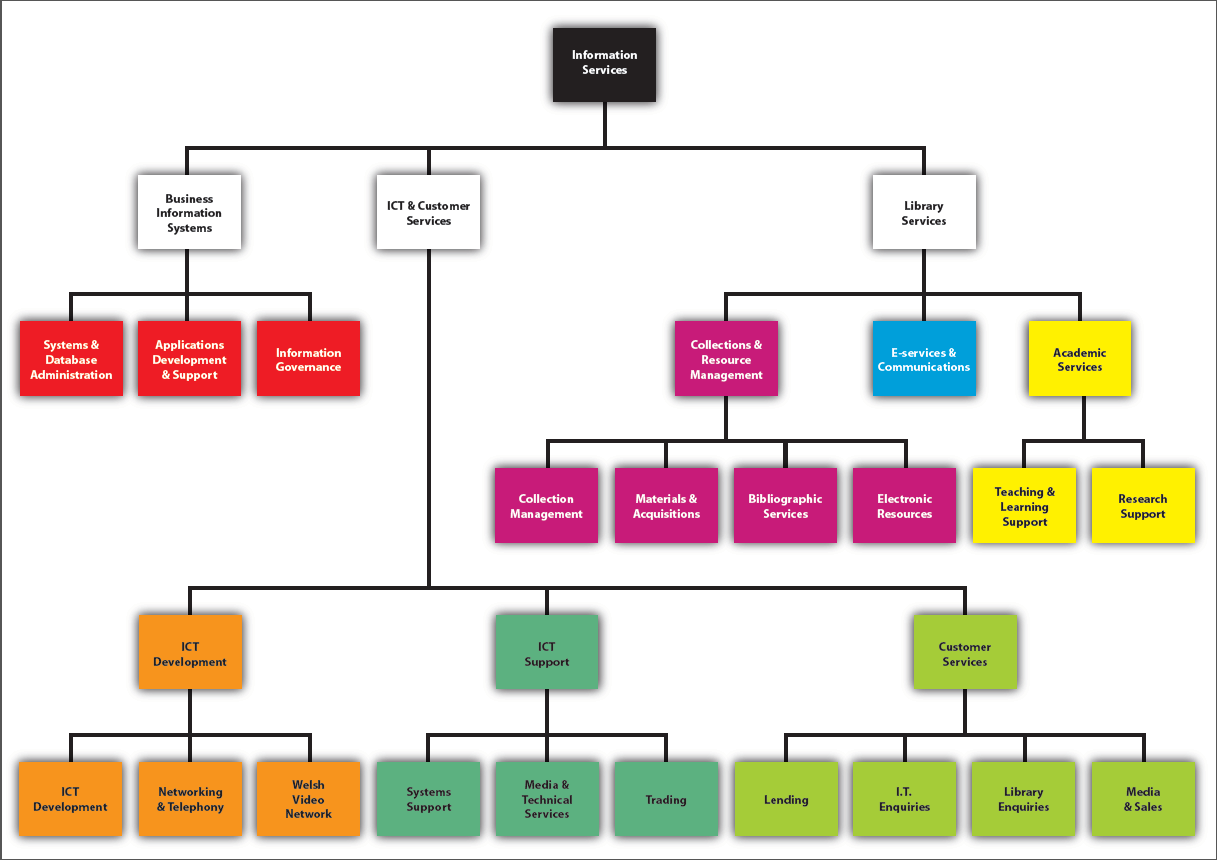
\includegraphics[scale=0.55]{./i-s-hierarchy-tree-march-2012}}
\caption{IS hierarchy tree}
\label{fig:i-s-hierarchy-tree-march-2012}
\end{figure}

IS department is located in Hugh Owen Building and takes over 40 \% of E floor.  Figure ~\ref{fig:isfloorplan} shows IS floor plan. Most of the IS staff are based in open plan office, with team leaders located in offices at the edges. Mine workplace was in workshop, which is a separate area from the main office.

\begin{figure}[H]
\centering
\centerline{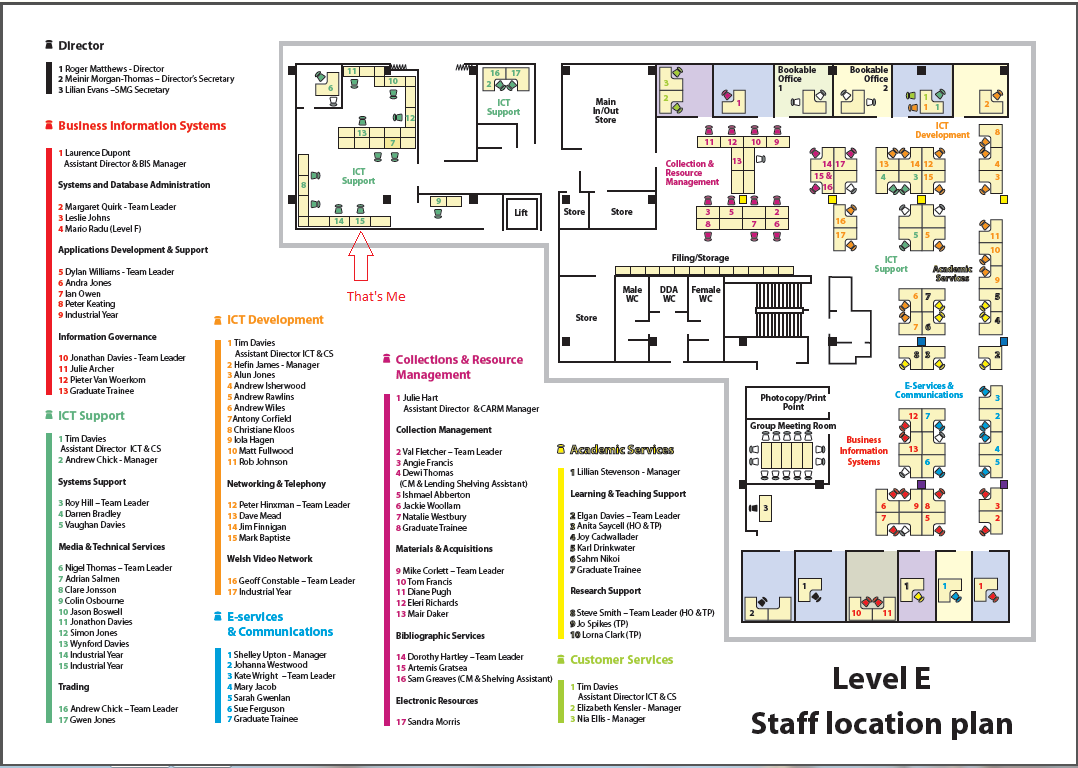
\includegraphics[scale=0.55]{./isfloorplan}}
\caption{IS Floor Plan \cite{ISFloor}}
\label{fig:isfloorplan}
\end{figure}

\section{ICT Support}
\subsection{Media \& Technical Services (My Team)}
The group that I am based in falls under IS $>$ ICT \& Customer Services $>$ ICT Support and is called "Media \& Technical Services". It is defined as a group responsible for the software and hardware upgrades and repairs a wide variety of ICT equipment types. It also provides multimedia services and supports ICT equipment within teaching spaces. All computer relevant hardware repairs are done within this group, it includes internal repairs (the equipment owned by university) as well as repairs for external customers (staff, students, members of publicity). The members of this group also provide technical support to the lecturers who are teaching and experience any issues with the teaching equipment. 

Computer workshop acts as a second line of contact for the customers and deal with complicated issues that could not be resolved in reasonable time frame by the help desk staff. IT Enquiries group deal with all incoming phone calls and emails. Usually over 90\% of all enquiries are resolved at this stage. If there is something that requires physical technician presence or problem can not be resolved remotely or at the help desk, then staff member opens new call in our job management system and assigns job to the appropriate team. That is how workshop team gets most of the jobs. Then jobs are distributed to the team members by our team leader or technicians pick up jobs themselves. Jobs that we receive vary greatly to each other, but mainly it is something that requires advanced knoweldge in IT, like laptop fix after spillage, not working printer, slow computer performance, virus removal, delivery and configuration of the new IT equipment, malfunctioned IT equipment diagnostics. We sometimes tend to get unusual jobs for which we either do not have appropriate equipment or non of us have appropriate qualification, I remember one job where it was requested to measure signal strength of the antenna, customer then was referred to some external company.

There are eight people working in Computer Workshop on permanent basis, one graduate trainee who joined us in January for one year fixed contract and two industrial year placement students like me, who work on rotating basis and change every year. Most of the full timers have relevant education, are A+ certified\cite{A+} and have previous experience in supporting IT. Computer workshop also does warranty and out of warranty repairs for Toshiba and Apple Inc computers, we have one technician who is Certified Apple Macintosh Technician. 

I would describe Workshop as relaxed work environment which allows all of us to talk freely to each other whilst remaining focused on our duties and completing assigned jobs. During first month I was trained by previous Industrial Year employees (they left at the end of our first month to continue with their studies), they showed me some systems that we use, helped to deal with my first jobs and provided with advice. After they left I could seek advice from anybody in the workshop, people were very friendly and helpful, they would explain all I need to do, although not mentioning some details which I had to find out by myself.
\subsection{Systems Support}
This group is responsible for all the aspects of PSV workstations, including software licensing, purchasing, management and implementation for Information Services and many departmental products. It makes backups for most of the University's systems and maintains two main server rooms, one in Penglais and one in Gogerddan. It also provides second/third line software support for the help-desk/workshop.
\subsection{Trading}
Offers a wide range of computers, laptops, media equipment and peripherals for sale to University Departments, individuals and external customers. Prices are generally competitive and are often at specially negotiated educational terms and/or with extended warranties for the members of the University,
\section{ICT Development}
Designs and implements systems and services for IS, other University departments, and external bodies. Also develops, implements, trains and supports IS users on bespoke software and ensures existing systems are efficient and cost effective. This includes Network and Telephone service design promoting standardization and centralization and managing improvements and information security incidents.
\section{Customer Services}
Provides Lending, ICT enquiries, Media \& Sales and Library Enquiry services for staff, students and visitors. Monitors the responsiveness and effectiveness of front-line services, ensures services best meet users' needs and promotes awareness of IS enquiry and front-line services. It also manages services and staffing for Freshers' Weekends and students' induction programmes.

\subsection{I.T Enquiries}
The first point of contact for face-to-face and online IT enquiries for all Information Services users. Troubleshoots any problems users experience with accessing or using Information Services services and resolves them or refers them as appropriate. Also supports the Public printing service, facilitates access to Information Services services such as email accounts, Aber cards, computing network, and printing and represents our users within IS e.g. presenting user feedback at meetings or user testing new services. I did two shifts a week on Service Point 2, helping customers with technical enquires and directing .

\section{BIS and Library Services}
There are also two other main groups called "Business Information Systems" and "Library Services". People in BIS are  responsible for development and support of the systems and processes required to maintain Admissions, Student Records, Finance, HR, Payroll and other associated business functions of the University. Library Services looks after all education materials: books, journals, articles as well as after education software systems like "AberLearn Blackboard".

\chapter{Technical environment}
When I just started my placement I was amazed by amount of different software used in IS and how information was spread across all these systems. At the beginning I was introduced to Interzone, Sunrise, Astra, Recall, SharePoint, Aber FAQs, Outlook, Voyager. All used to store different kind of information and help people with day-to-day duties. In this section I will go trough technical environment and will describe what software and tools I use while doing my job.
\section{Customers}
Majority of the IS customers are university staff and students, although from time to time we get requests from external bodies or private customers. All customers are with different amount of knowledges in IT, so sometimes I was finding myself explaining people how to efficiently use shortcuts on keyboard and stuff like that. Such difference in IT knowledge also required me to treat them differently, since not many of them would even understand what I mean if say that their hard drive is broken.

Usually when customer drops off their laptop in workshop or I collect broken computer, customer always want to know how quickly their fault will be fixed and try to be pushy about the time frame in which fault should be resolved. At the beginning it was a bit stressful since I was promising to 5 people at the same time that their fault fill be fixed in 1 to 3 days and then rushing to try and do job as quickly as I promised. Also it is bad approach because if I say that laptop will be fixed in 3 days and then some other more urgent jobs appear laptop definitely wont be ready by the time that I promised and when customer returns they are usually very unhappy and sometimes even angry. It lasted for a few weeks until I realized that there is nothing good in such approach and that I should concentrate on one fault instead of trying to fix ten of them at the same time. I stopped promising people about date when their equipment will be fixed, I am now trying to give blurred time frame so that customers do not expect to see their equipment back at least for a few days or weeks. I can work in more relaxed environment and do my job better w. 

Computer workshop provides almost the same service for staff, students and external customers in terms of ICT equipment repairs. If there is a lot of work, priority is given to the equipment owned by university. There is also difference in labour charge for different customers, equipment owned by university is repaired at smaller hourly rate and for external customers there is higher hourly rate charge. 
\section{My Work Environment (Computer Workshop)}
Computer Workshop is an open plan office as shown on ~\ref{fig:isfloorplan} with work benches and seating places at the walls and our team leaders office in the corner. When I started my placement I was given a place at the workbench and computer capable of doing simple office tasks. In computer workshop there are tools that you would expect to see in any more or less advanced household, this includes screwdrivers, pliers, soldiering kit, heat gun, drill, hex keys, different types of wrenches. However there are also some specific tools, that are used only for computer hardware diagnostic and repair: power adapters and PSUs (power supply units), PATA and SATA computer data cables, HDD cloners, magnifying glass to detect liquid damaged components, all of our workplaces have antistatic wrist straps and anti-static mats to prevent electrostatic discharge when working with sensitive computer components, network cable testers, multimeter. We also have store room where we keep new computer components such as new HDDs, cables, monitors, laptop screens, PSUs in case we need any of them during repair.    

Computer Workshop Technical Environment is probably most unusual in comparison to the rest of the IS. Here we not only deal with software related issues, but a hardware as well: soldiering, computer part replacement, cleaning after spillages, equipment shifting, hardware diagnostics, all unusual jobs come here. I will describe tools that I used most of all. 

When term starts we tend to get quite a lot of laptops that fail to boot in to the OS. Usually it is caused by damaged HDD, having broken sectors that can not be red. In such cases Diskology Disk Jockey PRO hard disk cloner\cite{DiskCloner} becomes extremely useful since it can skip broken sectors, filling them with zeros on the destination drive and making it possible to copy data from source drive. Some files may be damaged, but this is still better that frozen OS when it is impossible to copy any data at all. We also tend to get requests to restore lost data from USB pen drives and SD flash cards. In such case we use R-Studio, program which performs scan of the whole drive and then displays all data that is available for recovery. 

Symantec Ghost is disk cloning program, capable of making one-to-one copy of any storage media (HDD, SD Card, USB Pendrive). It can also copy just one partition of HDD or it can save disk/partition image as a file. Symantec Ghost is used heavily during Windows deployment on public computers. After reference Windows installation is complete and all necessary programs are installed, whole HDD is being captured in to the file, afterwards PSV computers join multicast session and image captured before is applied to all of the machines. It is very effective technique, sine there is no need to spend hours at each computer installing Windows with all corresponding applications required for education needs. Usually in one go we deploy image to 50-100 computers and our reference image size is around 50 GB(that is MS Windows 7, with almost 200 applications required for education) and that is when Symantec Ghost multicast ability becomes useful, because data is sent once to all computers and does not overload our network. Usually public PC is ready for use in 5-12 hours after deployment starts (depends on local network speed).

To remove viruses from the computers we use Sophos Endpoint Antivirus and Microsoft Security Essentials, both of these applications proved to be effective.
 
\section{Interzone}
All network equipment connected to the university network has its MAC address registered in our database, otherwise device will not get right IP address that would allow it to explore internet. To manage all these network records we use Interzone. 
Interzone is a front end web interface for the database that is used to manage records of network equipment in Aberystwyth University, it contains comprehensive information about the device, including information about the owner. 

On the main Interzone page it is possible to specify search criteria and look for devices that match request. Some of the search criteria are: IP address, MAC address, Owner's login, computer name. On the figure ~\ref{fig:main_interzone_page} there is main Interzone page.

\begin{figure}[H]
\centering
\centerline{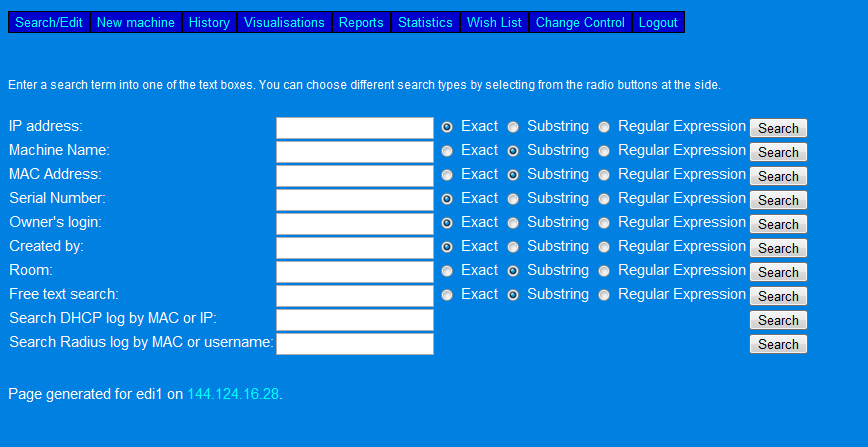
\includegraphics[scale=0.5]{./main_interzone_page}}
\caption{Main Interzone Page}
\label{fig:main_interzone_page}
\end{figure}

On figure ~\ref{fig:machine_record} Interzone record of my computer.

\begin{figure}[H]
\centering
\centerline{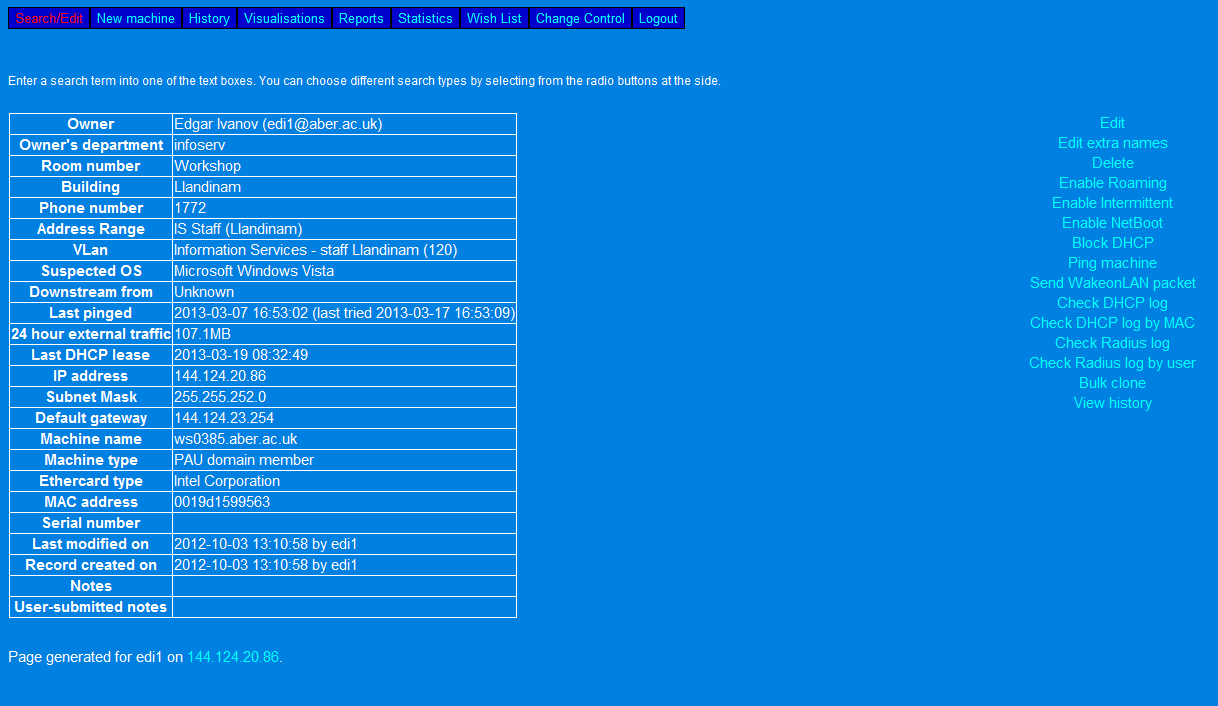
\includegraphics[scale=0.5]{./machine_record}}
\caption{Machine record}
\label{fig:machine_record}
\end{figure}

It contains various information about the owner, owners department, telephone number (if there is one), VLAN, IP and MAC addresses, you can also see who created this record and when it was last modified.

\begin{figure}[H]
\centering
\centerline{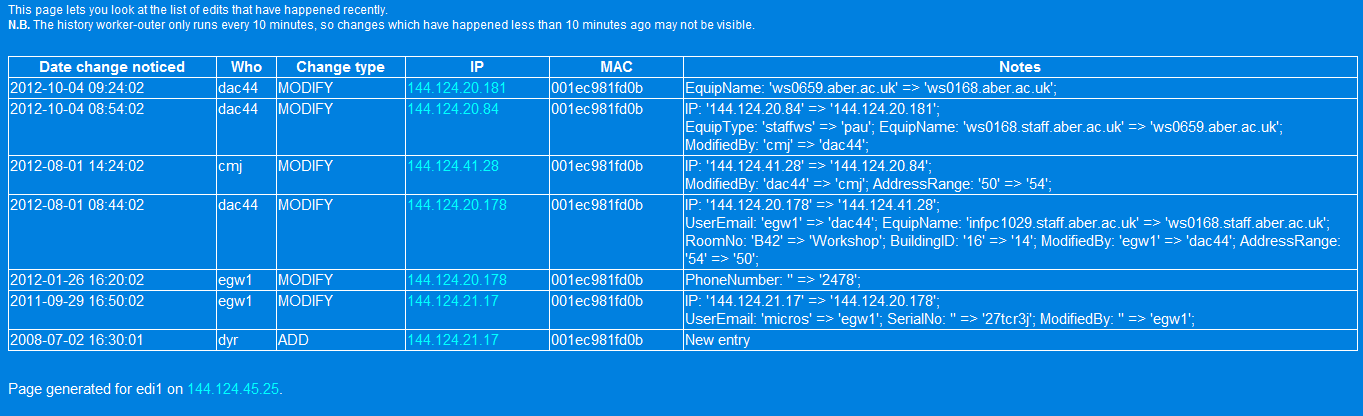
\includegraphics[scale=0.5]{./modification_history}}
\caption{Modification History}
\label{fig:modification_history}
\end{figure}

Information gathered from interzone can be very useful when troubleshooting computer connection issues. It is possible to check DHCP log to see if the computer gets IP address, look at the RADIUS logs that contain information about the user being successfully or unsuccessful in authenticating in out system. Figure ~\ref{fig:interzone_radius} shows RADIUS log for my mobile phone, where it is clearly seen that at some point in time I was unable connect to the network due to the authentication problem. When working on help desk and troubleshooting devices which were not connecting to the network properly, Interzone logs let me know what was going wrong so that I could choose appropriate solution. 

\begin{figure}[H]
\centering
\centerline{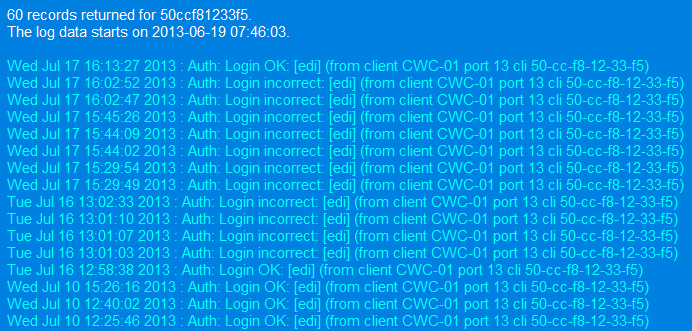
\includegraphics[scale=0.5]{./interzone_radius}}
\caption{RADIUS log}
\label{fig:interzone_radius}
\end{figure}

There are also interesting reports generated from information contained in database, on of them is on figure ~\ref{fig:interzone_statistics}, showing total amount of records in database.

\begin{figure}[H]
\centering
\centerline{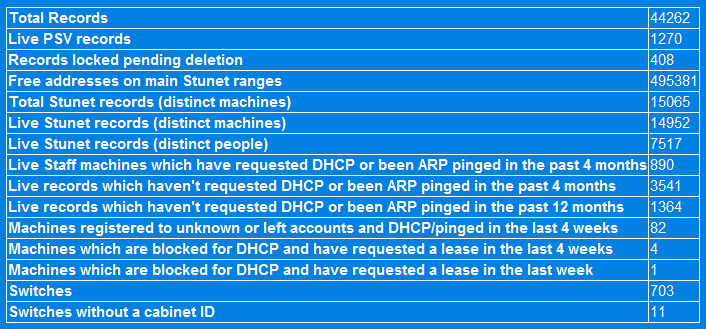
\includegraphics[scale=0.5]{./interzone_statistics}}
\caption{Interzone Statistics}
\label{fig:interzone_statistics}
\end{figure}

\section{Sunrise}
Sunrise is another front end web interface for the database that we use to keep track on current and past calls. This job management system is used to create new "jobs", allocate them to the technician or to the team, add comments about the job, send emails to the user with updates etc. Almost all jobs are coming to the Computer Workshop team from help desk, when first line fix is not possible new job is created with necessary information filled in. After job is assigned to my team our team leader assigns them to the technicians or, what happens more often, technicians themselves pick up a job to do from the list. On the figure ~\ref{fig:sunrise_main} you can see main Sunrise page, with all open and assigned to me jobs, as well as the boxes where it is possible to specify search criteria and search for the specific job.

\begin{figure}[H]
\centering
\centerline{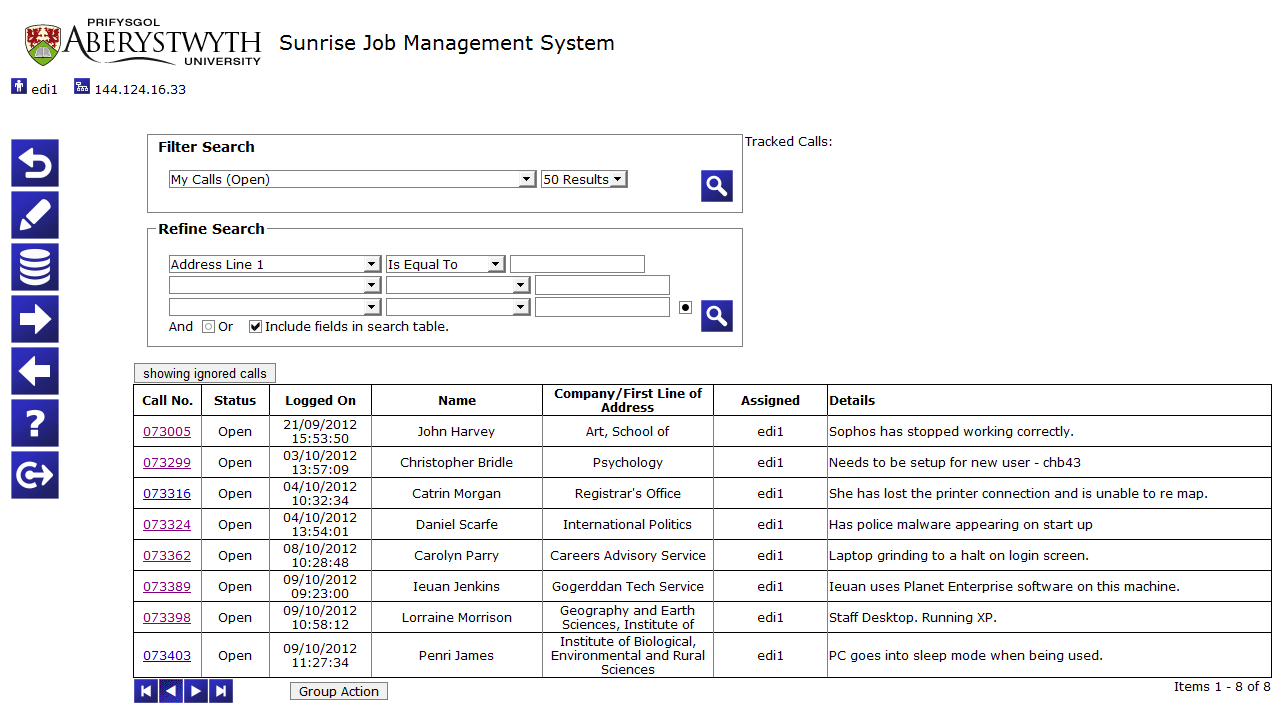
\includegraphics[scale=0.5]{./sunrise_main}}
\caption{Sunrise Main Page}
\label{fig:sunrise_main}
\end{figure}

Figure ~\ref{fig:sunrise_search} shows all the jobs that contain my email address "edi1" in them.

\begin{figure}[H]
\centering
\centerline{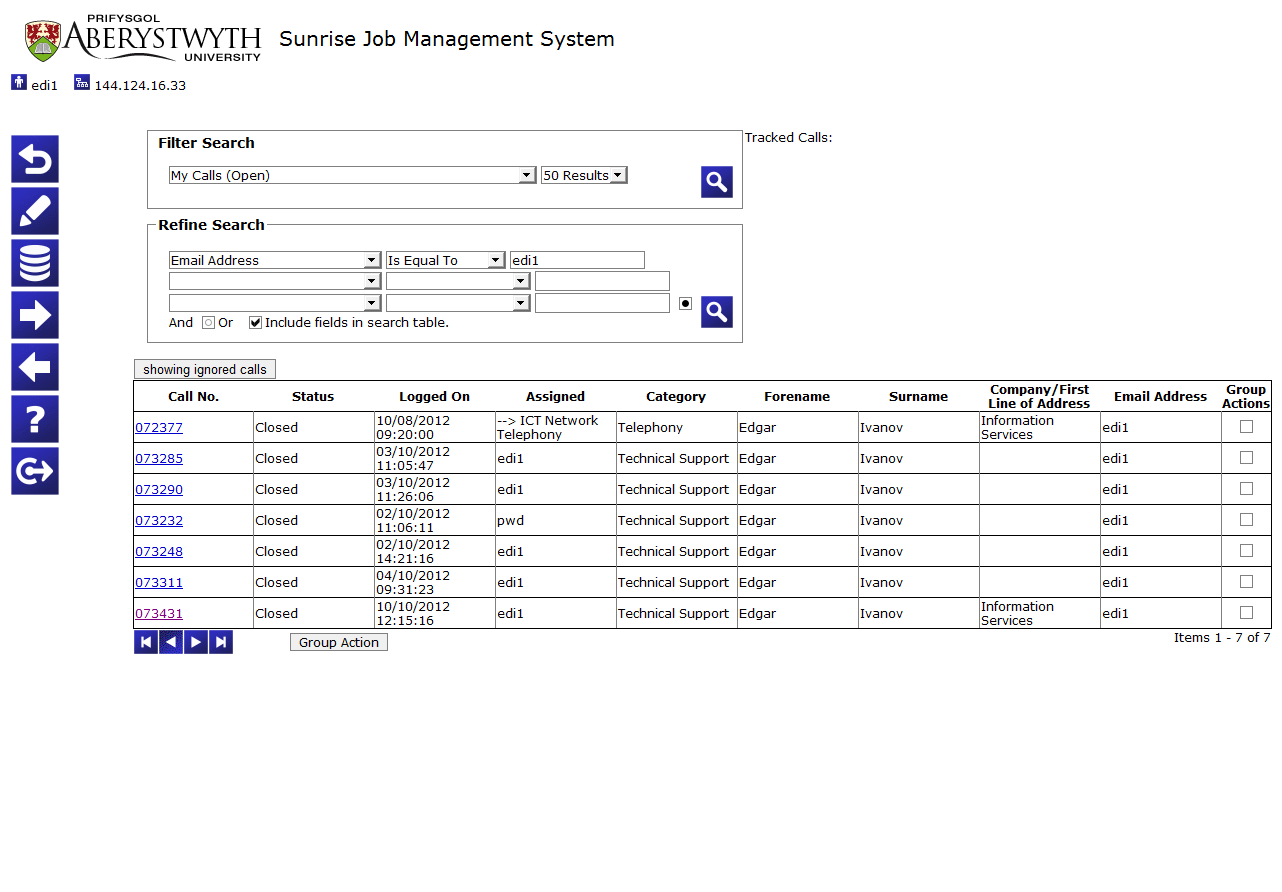
\includegraphics[scale=0.4]{./sunrise_search}}
\caption{Sunrise Search}
\label{fig:sunrise_search}
\end{figure}

Figure ~\ref{fig:sunrise_job} represents an ordinary job. Each job has a unique Call Number, in this case it is 075028, it also has the email address of the person who this job was opened for, phone number, address, equipment serial number, equipment description (laptop, desktop PC, projector, printer) and comments where an fault or issue is described. On the right hand side there is job history pane, each action that technician does must be added to the history so that if there will be any questions or issues in future it is possible to see what was done.

\begin{figure}[H]
\centering
\centerline{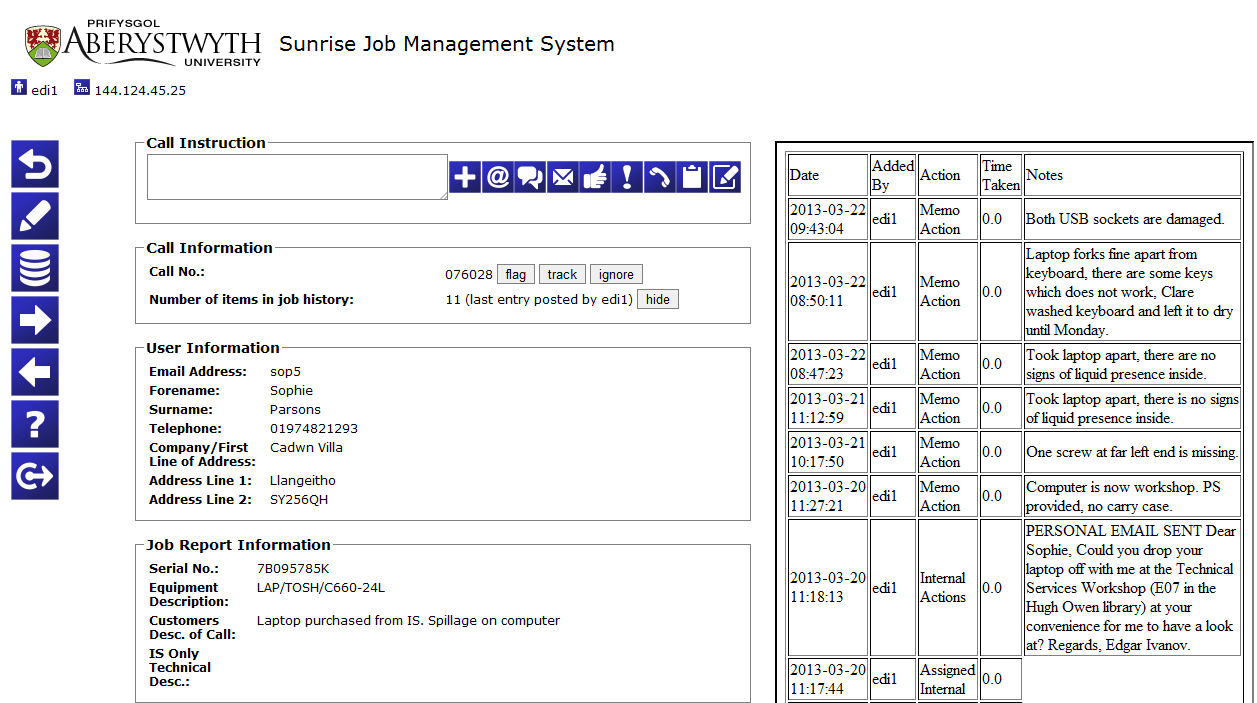
\includegraphics[scale=0.5]{./sunrise_job}}
\caption{Sunrise Job Record}
\label{fig:sunrise_job}
\end{figure}

\section{REG}
Whenever somebody becomes part of the university( students, staff, visiting staff) there is user account created for them. Username is allocated by the system an usually consists from three letters and some digits if required, mine for example was "edi1". Users then can use them to access their emails, e-journals, manage records about themselves and login to all the systems in university (if they were given access to them of course). To manage these accounts we have web interface called REG. I was using it mainly for unlocking user accounts while working on help desk, issuing new passwords, verifying identity of the people at the desk. On of the options I had was to make temporary password for any user, so that I could login as them to any system. It was quite useful when I needed to migrate user profile folder on Windows OS and user was away or it was not feasible for them to come in workshop to login. In such cases I would create temp password, login on the computer as them (that is when Windows creates actual folder for the user together with other corresponding registry entries), log off and revert password back, after all these steps I could copy all files from one machine to another and be sure that everything will work after machine will be delivered and user logon.
\section{SNMPc network manager}
Aberystwyth University is a large organization, having thousands of devices connected to its network. To provide reliable service to the end users we need to ensure that our network functions properly and issues are fixed as soon as possible. Network equipment such as: computers, printers, IP cameras, SALTO locks, wireless access points, VoIP phones all relay on ability to communicate (send/receive data), so it is crucial to ensure that there is working network connection at all times.  To monitor all our switches, routers, servers, workstations and printers IS uses program called SNMPc, developed by Castle Rock Computing. SNMPC is a Distributed Network Manager \cite{SNMPc} that uses SNMP protocol(Simple Network Management Protocol) to communicate and monitor devices. SNMPc makes it easier to look after whole network and network devices by identifying unresponsive equipment or network path with the issues and highlighting problematic devices on the network map. 

Figure ~\ref{fig:SNMPc_main} shows map of our network, each icon represents building, hall of residence or some separate piece of network, solid lines between icons represent fibre optics and thinner lines represents Gigabit Ethernet links. Green or purple icon shows that all nodes in them are contactable. If icon turns red it indicates that at least one node in this sub map is not contactable any more \cite{SNPMcSharePoint}. Buy just looking at the map it is possible to identify if there are any issues on the network and if there are try to fix them. I didn't use this application much since there are other people responsible for keeping our network up and running, but I found it quite interesting and useful to look at it time to time since I could see and explore our network in graphical view, what gave some insight of how corporate network should be configure and I will definitely use this knowledge in future at my workplace.

\begin{figure}[H]
\centering
\centerline{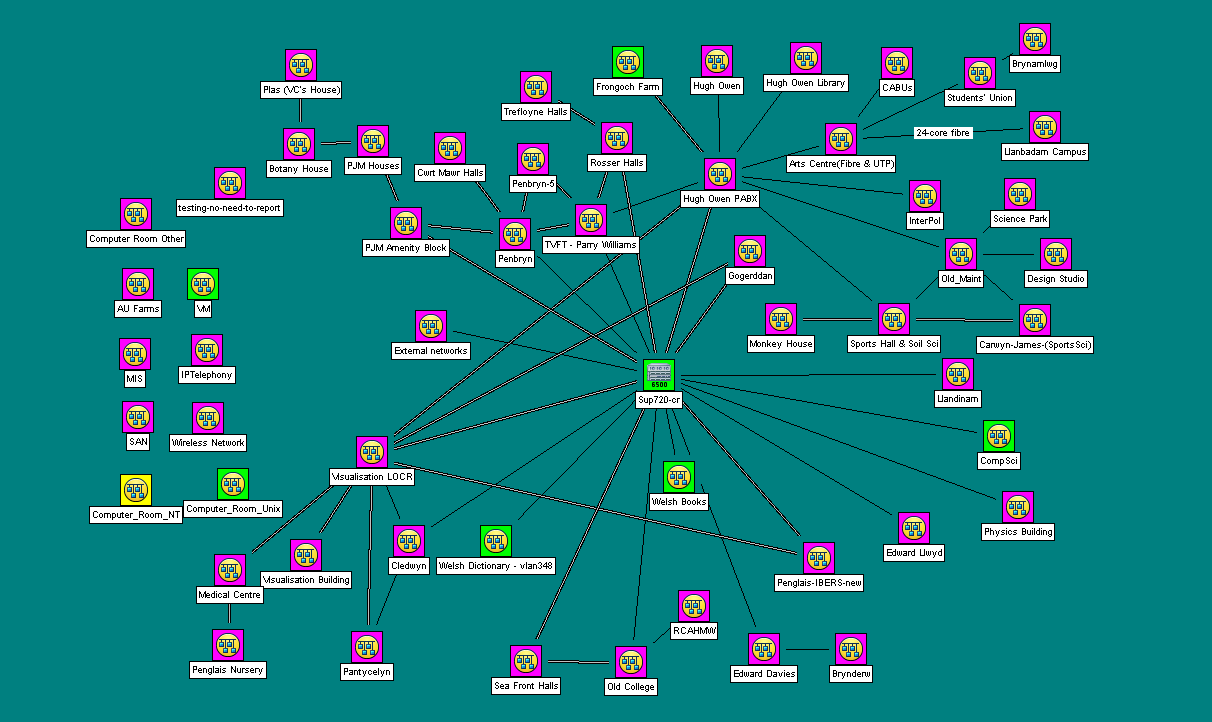
\includegraphics[scale=0.5]{./SNMPc_main}}
\caption{University network map in SNMPc application}
\label{fig:SNMPc_main}
\end{figure}

\section{Pcounter}
PCounter is an application that allows to  manage user print profiles. It allows to see print balance for everybody in university, it is possible to increase or decrease balance on the account, see print history and produce reports. I used it mainly for adding money to the user accounts when print credit machine was broken and users were coming to the desk to top up their account.
\section{VoIP Phones}
Right in the middle of my placement IS finished big project of VoIP phones roll-out in whole the university \cite{VoIP}. VoIP stands for "Voice over Internet Protocol" which means that voice data is carried over the Internet instead of public switched telephone network \cite{VoIP2}. There are numerous advantages of using VoIP phones over the usual ones, VoIP phones can display caller name acquired from the corporate directory, it has extension mobility which means that user can log in to any phone with their credentials, they allow for Voice Mail to be delivered to the users email Inbox. Most of the phones receive power over the Ethernet ("PoE") such approach eliminates the need for a nearby power outlet. When I was on calls in different departments and needed to make phone call to somebody in IS I found myself quite often using feature in phone that allows to find user phone number by their name. There is also possibility to install "softphone" software on the computer which allows to use computer and internet connection to make telephone calls instead of the usual handset and telephone line \cite{VoIP3}, it becomes very useful when staff works from home and have to receive phone calls from colleagues, so they are reachable on the same extension number as if they would be in the office. It is also possible to manage all phone aspects remotely with Cisco Unified Communications Manager. For such phones there is no need in dedicated Telephone Exchange equipment (which in Aberystwyth University used to occupy space of one living room), instead all it needs is software running on the server that handles all requests from the phones and manages whole phone infrastructure.  
\section{M drive}
"M" dive is known by University staff and students as a network file store, where users can keep any kind of information, the same as on USB pen drive and it is accessible from any computer that has access to the Internet. Size of file store is limited to 2 GB per user.  It is very convenient since information is stored on University server and there is no need to carry any physical media. IS makes regular backups of all "M" drives, so if user deleted something accidentally it is possible to recover file from the backup. When users logon on to the computers in the University computer rooms, filestore is automatically mapped on the computer as "M" drive \cite{MDrive}.

\section{Computers}
Here at Aberystyth University we have hundreds of computers used across campuses by both staff and students. While computers used by staff members may vary greatly in configuration, all public computers used by students have the same specifications across all campuses.
\subsection{PSVs}
Public Service Workstation computers that can use anybody who have University user account. IS manages around 500 public computers across campuses \cite{PSVs2}. We have two different versions of Optiplex 7010 computers. One model with higher specifications for teaching stations and USFF model for the student use. 

This summer we deployed new USFF Dell Optiplex 7010 \cite{PSVs} computers, since old ones were almost seven years old and didn't match current student needs in performance. All our PSVs run MS Windows 7 OS, there are more than 200 applications installed for academic use on them. PSV computers are configured to wipe everything straight away from "C" drive after user logs off, exception is only "D" drive where data is wiped every five days. Consequence of that is if user forgets to save document which he/she was editing on USB pen drive or somewhere else and logs of from the computer, they will lose data. This year senior management decided to change this and all user files will be redirected automatically to "M" drive, all standard MS Windows folders such as "My Document", "Pictures", MS Office auto save path etc, so hopefully there will be less student coming to the help desk and asking how it is possible to restore unsaved documents.
\begin{figure}[H]
\centering
\centerline{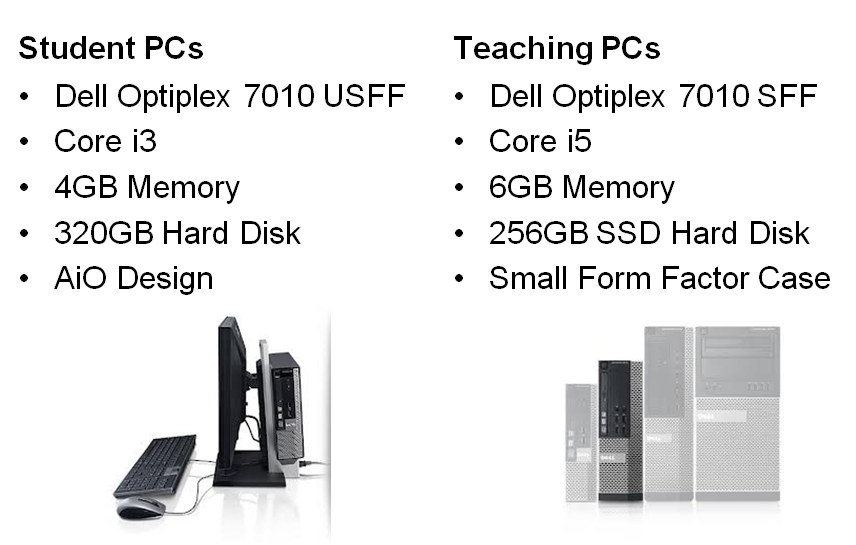
\includegraphics[scale=0.5]{./PSVs}}
\caption{Public workstation PCs \cite{PSVs}}
\label{fig:PSVs}
\end{figure}
\subsection{Staff Computers}
In Aberystwyth University departments are responsible for buying computers to their staff members, money for them are allocated from the departments budget. All such purchases go through IS. After IS is informed of computer choice, it goes through build process, which I will describe later, computer being prepared with all necessary software installed and joined to the domain. 

During my placement I was dealing with big variety of staff computers, most of them were standard tower PCs, with average hardware specifications, suitable for emails, videos, document editing and presentation preparation. Standard PC would be equipped with Intel� Core? Duo Processor (which is now more than six years old), from one to two GB of RAM, 80 - 250 GB HDD, integrated video card, running MS Windows: XP, Vista or 7. However across different departments I saw quite a lot of old PCs which were running Windows XP and hardly dealing with MS Office 2010 applications. Also there were some new Dell Optiplex computers, produced in last few years with quite good specifications.I also saw an old computer running OS/2, it was connected to some research equipment, reason for that one still being used is that there is no new software written for new operating systems and there is pretty much no choice, you either use it as it is, or not use.I have also dealt with wide variety of Apple Macintosh Computers, from low power Mac AirBooks to powerful Mac Pros which were used for image processing. The biggest amount of them (around 30) I saw in Geography department, where they were used to process large amounts of data. There is one interesting thing that I have noticed: during the whole year I haven't dealt with any staff computer that would be quipped with AMD processor. It frustrates me since AMD CPUs are cheaper due to competition on the market share between Intel and AMD(My own thoughts).

All in all computers seems to be fine for the purposes that they are used for, however some departments should really consider urgent upgrades. 

\section{Aber FAQs \& Sharepoint}
Aber FAQs is database of frequently asked questions, with answers to them. It is available to anybody on Internet and contains useful information on wide variety of questions. I used it mainly to remind myself of how to do certain things like computer connection to the university network, user account activation, email handler configuration etc. There is as well hidden part of this website which contains information only for IS staff. To access it user needs to provide username and password. Information in hidden part is relevant only to IS staff since in contains procedures with step-by-step guide and passwords required to complete tasks. It is organized in the same way as main website, having questions and then answers to them. I used it only a few times, when I had shifts on helpdesk, to create and activate new society account.

Sharepoint is described by Microsoft as collaboration platform \cite{Sharepoint}. In IS it is used primarily for content and document management. One of the features that I liked about Sharepoint is revision control capability, which allows to view older versions of the same document. Since anybody who has access to the document can change it and then save changes it may be handy to go back in time and see what changes were done and who exactly did them. On sharepoint IS staff keeps different documents relevant to their work. Some of the Staff Help Desk procedures are kept on Sharepont as well as on Aber FAQs, this is something that is going be changed in future, but nobody knows when it will happen. All Computer Workshop document are kept here as well. 

To provide bets experience for University lecturers workshop staff regularly visits all teaching rooms and checks for all equipment to work, this includes PC, DVD Player, Microphone, Video Camera, Projector, Speakers. After check is completed and everything works, whoever completed the check should update document on Sharepont were data about projector lamp hours is kept. This data is kept to determine how heavily projector is used and if any lamp should be replaced if it reaches end-of-life. Now I would like to describe how this update happens, person opens simple MS Excel spreadsheet, deletes old value and enters new one, then saves document. I personally was terrified by this approach to keep data. It would fine for some newbie at home to keep data in such way, but definitely not in serious organization as University. I would expect to see database, with simple front end, but not this. I saw a lot of such stupid things during my placement and I even get used to some of them so that now I could not even tell which way is right one. What I have learned from this is that sometimes it is useful to look fresh to things that you get used to do.      


\section{PSR2}
Here I would like to write some critics about computer workshop and our team leader as well. We have web application called PSR2 Maintenance where we keep information about computer room layouts with computer serial numbers. It is very simple web interface written with help of php and pulls data from the database. The only concern that I have is that this page is operating from one of the employees "M" drive. University provides such facility for all users to host their own web pages. All user needs to do is upload web site to special folder on "M" drive, change permissions and web site is available for the world. Drawback here is that if user account will be locked web page will not operate, it will display Not Found error message instead. 

On figure ~\ref{fig:main_PSR2_page} you can see main PSR2 page, which contains teaching rooms list that workshop technicians look after.

\begin{figure}[H]
\centering
\centerline{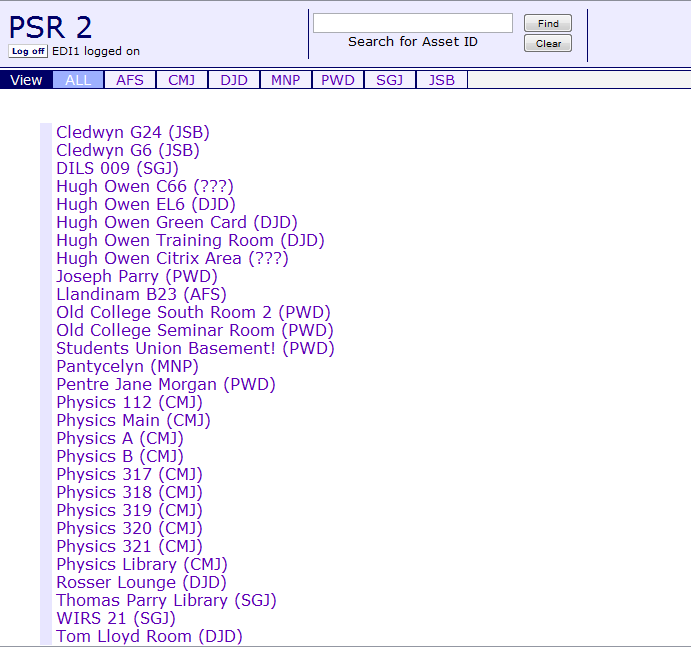
\includegraphics[scale=0.3]{./PSR2}}
\caption{Main PSR2 Page}
\label{fig:main_PSR2_page}
\end{figure}

Figure~\ref{fig:PSR2_SU_Room_layout} shows Students Union computer room layout, with computer names and serial numbers. Room comment holds code to unlock monitors from security straps. It also contains information when each computer was last time checked.

 It contains quite a lot of information, which is crucial to our work, and if for some reason account will be locked we will loose access to that information, which is at my knowledge is not held anywhere else.

\begin{figure}[H]
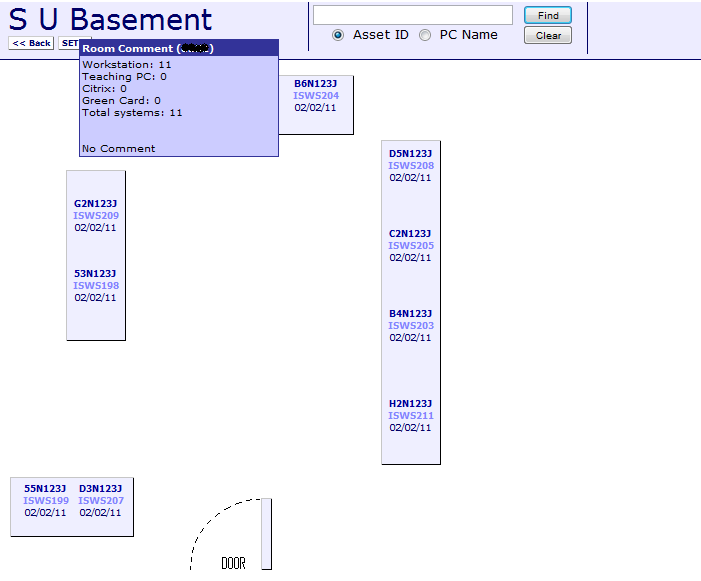
\includegraphics[scale=0.5]{./PSR2_SU_Room_layout}
\caption{PSR2 Students Union Computer Room Layout}
\label{fig:PSR2_SU_Room_layout}
\end{figure}

When I spoke to my college she explained my that this application was written for herself in first instance and then when our team leader accidentally saw it he asked for other workshop members to be added on the user list. That is how sometimes happens, no planning, ni testing, no official discussion.
\chapter{What I did}
Describe your 'routine' weekly duties. Spend a bit more time on areas where you have
responsibility or have put in effort e.g. summer builds, FAQS, summer course
registrations, any exploratory projects or mini-projects you may have been given to
name a few.

1 Room checks
When I joined IS I had to attend compulsory trainings for new staff. I was trained how to deal with customers in different situations, introduced to the rules and regulations as well as data protection act. Showed how to manage IS news channels as well as user records on reg and AStRA, how properly use Voyager - university library system. I was also shown how to use and provide support for Abercast, QMP, Qwizdom - these are applications and tools used by lecturers to provide better experience for the students during lectures. I also learned many more other little things while doing jobs and providing support to the customers.

My work hours are from 8:30 until 17:00 Monday to Thursday and on Fridays we work one hour less, until 16:00. Since I live just a few kilometres away from the university I get to work by walk and it usually takes me around 15 min. My day starts from assigned jobs review. I open Sunrise - our job management system and look through all jobs assigned to me, them then decide and plan what to do during the day (it is good since I have freedom and what to do, when and how, it allowed me to develop my own techniques of fixing problems, although I missed some procedures and guidelines for certain situations).

There are two main types of the jobs that I do, those that I can do in the workshop and those were I need to visit customer. After I read fault description I decide whether job can be done on customers site or in the workshop. Usually software faults require physical technician presence since if job appeared in our database it means that first line fix was not available or impossible. With hardware faults everything is much simpler, I just go, pick up faulty equipment and bring to the workshop. With laptops I always send email to the customer asking he/she to bring laptop to the workshop. Whether it simple software problem or some hardware issue I always contact customer and arrange time when I can come and fix problem or pick up faulty equipment. Sometimes software problems may be difficult and after few hours of trying to fix it on site I decide to bring computer with me to the workshop where in more relaxed environment I can look for fix or ask advice my colleagues.


\chapter{Critical evaluation}
\section{Becoming Mac Technician}
\bibliographystyle{ieeetr}
\bibliography{bibl}

\end{document}